\documentclass{article}
\usepackage{iclr2027_conference,times}
\usepackage{natbib}
\usepackage{booktabs}
\usepackage{graphicx}
\usepackage{amsmath,amsfonts,amssymb,amsthm}
\usepackage[norelsize,ruled,vlined,linesnumbered]{algorithm2e}
\SetAlFnt{\normalsize}
\SetAlgoNlRelativeSize{0}
\usepackage{xcolor}
\usepackage{hyperref}
\usepackage{cleveref}
\usepackage{float}
\crefname{algocf}{algorithm}{algorithms}
\Crefname{algocf}{Algorithm}{Algorithms}
\crefname{assumption}{assumption}{assumptions}
\Crefname{assumption}{Assumption}{Assumptions}
\usepackage{xspace}

\hypersetup{colorlinks,hypertexnames=false,linkcolor={blue!90!black},
  citecolor={blue!90!black},urlcolor={blue!80!black}}

\newcommand{\bR}{\mathbb{R}}
\newcommand{\bE}{\mathbb{E}}
\newcommand{\bP}{\mathbb{P}}
\newcommand{\bQ}{\mathbb{Q}}
\newcommand{\Var}{\operatorname{Var}}
\newcommand{\Cov}{\operatorname{Cov}}
\newcommand{\eps}{\varepsilon}
\newcommand{\cS}{\mathcal{S}}
\newcommand{\cA}{\mathcal{A}}
\newcommand{\cM}{\mathcal{M}}
\newcommand{\wt}{\widetilde}
\newcommand{\wh}{\widehat}
\newcommand{\ie}{\textit{i.e.}\@\xspace}
\newcommand{\eg}{e.g.\@\xspace}
\newcommand{\iid}{i.i.d.\@\xspace}
\newcommand{\abs}[1]{\lvert #1 \rvert}
\newcommand{\prn}[1]{\left( #1 \right)}
\newcommand{\set}[1]{\left\{ #1 \right\}}
\newcommand{\ind}[1]{\mathbf{1}\!\left\{#1\right\}}
\newcommand{\method}{StableMax-PPO}

\DeclareMathOperator*{\argmax}{arg\,max}
\DeclareMathOperator*{\argmin}{arg\,min}
\newtheorem{proposition}{Proposition}
\newtheorem{theorem}{Theorem}
\newtheorem{lemma}{Lemma}
\newtheorem{corollary}{Corollary}
\theoremstyle{definition}
\newtheorem{definition}{Definition}
\newtheorem{assumption}{Assumption}
\theoremstyle{remark}
\newtheorem{remark}{Remark}
\setlength{\parindent}{0cm}
\addtocontents{toc}{\protect\setcounter{tocdepth}{0}}

\title{StableMax-PPO: Finite-Budget RLHF with a Max--Stability Trade-off}
\author{}
\date{}

\begin{document}
\maketitle

\begin{abstract}
Reinforcement learning from human feedback (RLHF) has substantially
improved language-model post-training, but many RLHF pipelines optimize
the expected reward of a single response even when deployment selects
the best from a finite set. Recent Best-of-\(N\)-aware methods reduce
this mismatch, yet many operate on scalar rewards or nominal reward-model
distributions, discarding the ordinal threshold structure that determines
the maximum and leaving upper-tail optimization sensitive to calibration
error, degradation of typical responses, and policy drift. To address
these limitations, we introduce \textbf{\method{}}, which directly trains
the policy for the same finite-budget maximum used at deployment while
retaining the predictive distribution of a frozen ordinal reward model
trained from repeated human ratings. A one-sided envelope on its CDFs
yields the exact worst-case Best-of-\(N\) objective over the resulting
ambiguity set, and the same threshold construction provides an exact
response-level credit for PPO optimization. Nominal-mean and independent-quality floors guard against degradation
of typical responses and target-evaluator over-optimization, while
reference-policy KL control and state-complete rollback constrain
excessive policy updates. Across
three seeds, \textbf{\method{}} retains competitive finite-budget maximum
performance while reducing held-out drift relative to baselines,
characterizing a calibration-robust, lower-drift operating point on the
max--stability frontier.
\end{abstract}
\section{Introduction}
\label{sec:introduction}

Many language-model systems generate several responses and return, rerank, or
inspect the best candidate, while common RLHF objectives optimize the expected
score of one response.  The distinction matters because a mean improvement need
not increase the chance of obtaining a strong candidate within a fixed budget.
Mean-PPO and GRPO remain effective general-purpose post-training methods
\citep{shao2024deepseekmath,guo2025deepseekr1}, and recent max@\(k\),
Best-of-\(N\), and inference-aware policy-gradient methods better align training
with finite-budget deployment
\citep{chow2025inference,tang2025inference,walder2025pkpo,
bagirov2025best,li2026posttraining,poiani2026maxk}.  We do not claim the first
finite-budget objective.  The unresolved setting is an imperfect ordinal
evaluator: collapsing its output to a scalar discards the threshold
probabilities that determine the maximum, while optimizing a nominal upper tail
can amplify calibration error, sacrifice typical quality, or move the policy
far from its reference.  Our question is therefore how to optimize the same
finite-budget statistic used at deployment while preserving the evaluator's
ordinal information and keeping quality and drift independently measurable.

We introduce \method{}, an evaluator-to-optimizer construction for this
setting.  A frozen ordinal Moment RM, trained from repeated HelpSteer2
helpfulness ratings \citep{wang2024helpsteer2}, represents conditional rating
disagreement as a predictive distribution over \(\{0,1,2,3,4\}\).  The
distribution retains every threshold event used by the maximum; its mean
provides an ordinary model-implied quality measure, while its variance is kept
as a disagreement diagnostic rather than a reward bonus.  We place a one-sided
calibration envelope on the CDFs in the direction adverse to upper-tail
performance.  The resulting product distribution exactly attains the
worst-case Best-of-\(N\) value over the declared ambiguity set, and the same
threshold products yield an exact response-level marginal credit for policy
optimization.

This shared construction is the main technical distinction: calibration
robustness changes both the deployment-level group objective and the credit that
differentiates it, rather than entering as an auxiliary penalty.  PPO is only
the optimization carrier.  A nominal-mean floor and a separately trained,
frozen Quality RM from preference pairs guard typical responses and transfer
beyond the target evaluator; reference-policy KL
regularization and state-complete rollback control the accepted update
trajectory.  The robust maximum, both quality measurements, and policy drift
consequently remain separate quantities, making the max--stability trade-off
observable rather than hiding it in a weighted reward.

The central contribution is therefore an evaluator-to-gradient contract, rather
than a new PPO optimizer in isolation or an additive list of stabilization
heuristics.  Existing finite-budget objectives can be optimized with a scalar
reward, but that scalarization happens before the group interaction is
differentiated.  Here the adverse CDF envelope first defines the deployment
functional and then induces the response-level credit used by PPO.  Calibration
robustness consequently changes both what counts as a successful group and
which response receives credit, while the quality and KL mechanisms remain
separately auditable.

Our contributions are:
\begin{itemize}
\item \textbf{A calibration-robust ordinal objective.}  We derive the exact
finite-\(N\) worst-case maximum over a one-sided product ambiguity set and
quantify its dependence on envelope coverage and radius.
\item \textbf{An exact group-to-response credit.}  The same threshold
construction gives a Rao--Blackwellized marginal credit whose score-function
expectation is the gradient of the robust group objective and whose credits are
computable in \(O(N|\mathcal R|)\) time.
\item \textbf{A controlled optimization realization.}  We combine this credit
with PPO while keeping nominal mean, independently evaluated quality, KL, and
rollback as distinct safeguards rather than redefining the robust reward.
\item \textbf{An empirical characterization of the operating frontier.}  At
\(N=32\) across three seeds, \method{} attains a competitive robust maximum with
lower held-out drift than Mean-PPO, GRPO, and Scalar max-PPO; max-oriented
comparators attain higher maxima at greater drift.
\end{itemize}

\section{Problem Setup}
\label{sec:problem-setup}

\subsection{Setting and assumptions}
We study response-level RLHF with a fixed Best-of-\(N\) generation budget.  The
policy parameter \(\theta\) is trainable, whereas the ordinal Moment RM \(\omega\),
scalar Quality RM \(\eta\), and reference policy \(\pi_{\rm ref}\) are frozen.
For \(x\sim\mathcal D\), responses factor as
\(\pi_\theta(Y\mid x)=\prod_h\pi_\theta(a_h\mid x,a_{<h})\), and a rollout
contains \(Y_{1:N}\overset{\mathrm{iid}}{\sim}\pi_\theta(\cdot\mid x)\).  We
assume (A1) conditional independence of rating outcomes across candidates, (A2)
frozen evaluators, and (A3) the differentiability and likelihood-ratio
regularity needed below.  Thus changes in the measured frontier are attributable
to the policy and controller rather than to a moving evaluator.  Each response
receives one terminal evaluation; the group statistic is formed before any
response-level credit is assigned.

Assumption (A1) concerns annotation outcomes conditional on completed
responses; it does not assert token independence.  It is what converts each
threshold event for the maximum into a product of candidate CDFs.  Assumption
(A2) keeps both evaluators and the reference policy fixed, so the measured
frontier moves only through the policy and controller.  Assumption (A3) enables
the likelihood-ratio differentiation in Theorem~\ref{thm:main-gradient}.
Correlated evaluator errors are therefore outside the product model rather than
an effect absorbed by the optimizer.

\subsection{Ordinal evaluator and finite-budget value}
The Moment RM returns \(p_{\omega,r}(x,y)=\Pr_\omega(R=r\mid x,y)\) for
\(\mathcal R=\{0,1,2,3,4\}\); write \(\Delta(\mathcal R)\) for the probability
simplex on these five levels.  Its mean
\(\mu_\omega=\sum_r rp_{\omega,r}\) measures target-RM quality, while
\(\sigma_\omega^2=\sum_r(r-\mu_\omega)^2p_{\omega,r}\) is retained only as a
model-based disagreement diagnostic; the independent scalar \(Q_\eta(x,y)\) is a
separate quality check.  The category endpoints are fixed by the training data;
the ordinal-probit parameterization is given in Appendix~\ref{app:theory}.
Thus the five levels are part of the evaluator interface rather than thresholds
selected after observing policy outcomes.  The mean, categorical vector, and
variance have distinct roles: only the vector determines the finite-budget
target, and the variance remains diagnostic rather than becoming a reward bonus.

For candidate \(j\), let \(F_{\omega,j}(t)=\sum_{r=0}^{t}p_{\omega,r}(x,Y_j)\).
Under (A1), the nominal finite-support identity is
\(h_N^{\rm nom}=\sum_{t=1}^{4}[1-\prod_{j=1}^{N}F_{\omega,j}(t-1)]\), and
\(J_N^{\rm nom}(\theta)=\mathbb E[h_N^{\rm nom}]\).  Its threshold products
show why the full ordinal vector matters: a candidate is useful when the other
responses leave a threshold uncovered, which a scalar maximum cannot represent
before credit assignment.  The identity integrates out rating noise exactly;
the top-rating event is only one of the four threshold terms.  Two responses
with the same predictive mean can therefore have different group value because
their mass is distributed differently across thresholds.

We estimate \(\varepsilon_{\rm cal}\) on independent prompt clusters before
training (Appendix~\ref{app:theory}) and use the one-sided envelope
\(\overline F_j(t)=\min\{1,F_{\omega,j}(t)+\varepsilon_{\rm cal}\}\), with
\(\overline p_{j,r}=\overline F_j(r)-\overline F_j(r-1)\).  Define
\(\mathfrak U_{\varepsilon_{\rm cal}}(p_{\omega,1:N})
:=\prod_{j=1}^{N}\{q_j\in\Delta(\mathcal R):
F_{q_j}(t)\le\overline F_j(t),\ t=0,\ldots,3\}\).  Set
\(\overline F_j(-1)=0,\overline F_j(4)=1\).  Increasing a CDF is adverse to an
upper-tail maximum, so the envelope changes the deployment target and its
policy credit together; it is not an auxiliary reward bonus.  The radius is
estimated on a split disjoint from policy training, so it fixes a declared
conservatism level before policy outcomes are observed rather than tuning a
reward after the fact.

\subsection{Robust constrained objective}
The robust group value is
\(h_N^{\rm rob}:=\inf_{q_{1:N}\in\mathfrak U_{\varepsilon_{\rm cal}}(p_{\omega,1:N})}
\mathbb E_q[\max_jR_j]=\sum_{t=1}^{4}[1-\prod_{j=1}^{N}\overline F_j(t-1)]\).
Our single optimization objective is
\begin{equation}
\label{eq:robust-max-closed}
\begin{aligned}
\max_{\theta}\quad J_N^{\rm rob}(\theta)
&:=\mathbb E[h_N^{\rm rob}(x,Y_{1:N})],\\[-1pt]
\text{s.t.}\quad &M(\theta):=\mathbb E[\mu_\omega(x,Y)]\ge m_0,\quad
Q(\theta):=\mathbb E[Q_\eta(x,Y)]\ge q_0,\\[-1pt]
&K(\theta):=\mathbb E_x[\mathrm{KL}(\pi_\theta\Vert\pi_{\rm ref})]\le\delta .
\end{aligned}
\end{equation}
The floors \(m_0,q_0\) are fixed from the reference policy and keep target-RM
and independent quality visible, while \(K\) measures policy motion separately.
In PPO, the floors enter through dual credits, the KL term through the
surrogate, and the distinct threshold \(\delta_{\rm hard}\) through batch
rollback; the measured token KL is an acceptance statistic, not a population
trust-region guarantee.  This separation makes a change in the reported
maximum attributable to the robust target distinguishable from a change caused
by a quality multiplier or by the update-acceptance rule.  In particular, the
independent Quality RM is a transfer check trained from preference pairs, not
another term that can be traded against the robust maximum; the multipliers only
price violations of the declared floors.

\section{Method}
\label{sec:method}

The method separates the deployment target from its stabilizers.  The target
is the robust ordinal maximum; the stabilizers control typical quality and
policy motion.  This separation makes the max--stability trade-off visible
instead of hiding it in a scalar reward weight.  The construction has two
steps: first, the evaluator distribution is transformed into a worst-case
finite-budget functional; second, that functional is differentiated into
response-level credits and carried by PPO.  The theorems below establish these
steps before the implementation details introduce clipping, dual prices, and
rollback.

\subsection{Exact robust maximum and marginal credit}
\label{subsec:exact-credit}

\begin{theorem}[Exact finite-budget robust maximum]
\label{thm:main-max}
Under (A1), for every fixed \((x,Y_{1:N})\), an optimizer over the product
ambiguity set is \(q_j=\overline p_j\) for every \(j\), and the attained
worst-case Best-of-\(N\) value is
\begin{equation}
\label{eq:robust-max-theorem}
\inf_{q_{1:N}\in\mathfrak U_{\varepsilon_{\rm cal}}(p_{\omega,1:N})}
\mathbb E_q[\max_jR_j]
=\sum_{t=1}^{4}\left[1-\prod_{j=1}^{N}\overline F_j(t-1)\right].
\end{equation}
\end{theorem}

The key point is simultaneous optimality.  The maximum is coordinatewise
increasing, so saturating every admissible CDF upper bound makes all candidates
stochastically smallest at once; the adversary need not choose a different
perturbation for each threshold.  The full ambiguity-set problem therefore
reduces to four threshold products, without rating sampling or enumerating
\(5^N\) joint outcomes.  This is stronger than applying a separate correction
to a scalar maximum: the same envelope is feasible for the entire product set
and is extremal for all thresholds simultaneously.

For a candidate \(i\), let \(\overline R_i\sim\overline p_i\) and
\(\overline M_{-i}=\max_{j\ne i}\overline R_j\).  Its leave-one-out marginal
credit is
\begin{equation}
\label{eq:robust-credit-closed}
q_i^{\rm rob}:=\mathbb E[(\overline R_i-
\overline M_{-i})_+\mid x,Y_{1:N}]
=\sum_{t=1}^{4}[1-\overline F_i(t-1)]\prod_{j\ne i}\overline F_j(t-1).
\end{equation}
The first factor is candidate \(i\)'s probability of crossing threshold \(t\);
the product over \(j\ne i\) is the probability that the other responses leave
that threshold uncovered.  This leave-one-out value captures incremental group
credit rather than a winner indicator, so a response can matter without having
the largest mean score.  Prefix and suffix products compute all credits in
\(O(N|\mathcal R|)\) time per prompt using the same kernel as the group
objective, without sampling latent ratings.  In particular, a high-mean response
can receive little marginal credit when other candidates already cover the same
thresholds, while a complementary response can receive credit without being the
mean-score winner.  The credit therefore preserves the group interaction that
would be lost by assigning each response an isolated scalar reward.  It is a
marginal, rather than additive, decomposition: ties or redundant candidates
need not exhaust the group value, because the signal is intended to measure
incremental threshold coverage.

This distinction also determines what is held fixed in the comparison.  The
candidate responses are sampled from the policy, but the rating randomness is
integrated analytically; changing \(N\) would change the group functional, not
merely the number of reward observations.  At the fixed budget used here, the
credit is therefore aligned with the deployment statistic at the level of both
its value and its derivative.

\begin{theorem}[Exact marginal policy credit]
\label{thm:main-gradient}
Under (A1)--(A3), the exact group objective has the score-function gradient
\begin{equation}
\label{eq:robust-policy-gradient}
\nabla_\theta J_N^{\rm rob}(\theta)=\mathbb E\left[
\sum_{i=1}^{N}q_i^{\rm rob}\nabla_\theta\log\pi_\theta(Y_i\mid x)\right].
\end{equation}
Thus the response-level estimator is unbiased before PPO clipping.
\end{theorem}

This is the evaluator-to-policy bridge: latent rating draws are integrated out,
while the likelihood ratio distributes each candidate's threshold credit over
its tokens.  The same cached categorical probabilities define the robust target
and every leave-one-out credit; PPO supplies only the clipped optimization
carrier.  Before clipping, no sampled rating estimator or learned group-winner
critic is needed.  After clipping, the estimator is an implementation of the
same credit rather than a new objective; clipping and rollback are explicit
controls on the accepted optimization trajectory.  Thus the exact identity
specifies the target gradient, while the PPO ratio, KL coefficient, and
acceptance test specify only how aggressively that gradient is realized.  This
also clarifies the empirical attribution: a difference in the robust endpoint
is a change in the evaluator-defined target, whereas a difference in held-out
KL or rollback frequency reflects the controller's operating point.

\subsection{Constrained PPO update}
\label{subsec:constrained-credit}

For dual variables \(\lambda_m,\lambda_q\ge0\), the response-level credit used
by PPO is
\begin{equation}
\label{eq:constrained-credit}
\widetilde q_i=q_i^{\rm rob}+\frac{\lambda_m}{N}\mu_\omega(x,Y_i)
 +\frac{\lambda_q}{N}Q_\eta(x,Y_i),\qquad
A_i=N[\widetilde q_i-b_\psi(x)].
\end{equation}
The factors \(1/N\) match the one-response constraints to the group objective;
the prompt-only baseline preserves the score-function identity.  We use the
standard clipped PPO surrogate and full-categorical token KL.  Writing
\(\rho_{i,h}=\pi_\theta(a_{i,h}\mid s_{i,h})/
\pi_{\rm old}(a_{i,h}\mid s_{i,h})\), the update maximizes the standard
per-token expression \(\min\{\rho_{i,h}A_i,
\operatorname{clip}(\rho_{i,h},1-\epsilon_{\rm PPO},1+\epsilon_{\rm PPO})A_i\}\)
averaged over candidates, minus \(\beta_{\rm KL}\widehat{\mathrm{KL}}\), and divides
by the lagged RMS scale.  The full implementation, including projected dual
updates, is specified in Appendix~\ref{app:algorithm}.

Before a tentative step, \method{} snapshots all policy parameters and the
complete optimizer state.  If the post-update KL on the same rollout states
exceeds \(\delta_{\rm hard}\), both snapshots are restored; baseline, dual,
RMS, and controller states advance only after acceptance.  Snapshotting the
optimizer moments is necessary for Adam-like optimizers, and the resulting
rollback count is comparable across baselines under the shared controller.
The soft target \(\delta\) and the hard threshold \(\delta_{\rm hard}\) serve
different purposes: the former is the reference-policy constraint represented
by the KL controller, whereas the latter is a batch-level reject rule.  An
accepted update can still differ from the population-constrained optimum, which
is why held-out KL is measured independently rather than inferred from the
rollback threshold.

\subsection{StableMax-PPO}
\label{subsec:algorithm}
Here \(\mathsf{Opt}\) denotes the complete policy-optimizer state, including
momentum and adaptive-variance buffers.  We compute
\(\widehat{\mathrm{KL}}\) as the batch mean of the full-categorical token KL on
rollout states, not from sampled actions.  The update uses \(q_i^{\rm rob}\) and
\(A_i\) from \cref{eq:robust-credit-closed,eq:constrained-credit}.  Starting
from the current policy and controller state, each iteration evaluates only the
frozen models on a fixed-size rollout; the policy and controller are updated,
whereas the models, calibration radius, floors, soft target \(\delta\), and hard
rollback threshold are fixed by the protocol.
\begin{algorithm}[H]
\caption{StableMax-PPO update}
\label{alg:stablemax}
\KwIn{Prompts \(x\sim\mathcal D\); initial trainable policy \(\pi_\theta\);
frozen \(p_\omega,Q_\eta,\pi_{\rm ref}\); fixed \(N,\varepsilon_{\rm cal},
m_0,q_0,\delta,\delta_{\rm hard}\).}
\KwOut{Accepted policy parameters and optimizer/controller state.}
Initialize \(\mathsf{Opt}\), \(b_\psi\), \(\lambda_m,\lambda_q\),
\(\beta_{\rm KL}\), and lagged RMS scale \(s\)\;
\For{$k=1,\ldots,T_{\rm pol}$}{
  Set \(\pi_{\rm old}\leftarrow\pi_\theta\) and roll out \(N\) responses per
  prompt; evaluate the frozen \(p_\omega,Q_\eta\)\;
  Compute \(q_i^{\rm rob}\) from \cref{eq:robust-credit-closed} and \(A_i\)
  from \cref{eq:constrained-credit}\;
  Snapshot \((\theta,\mathsf{Opt})\) and take one clipped-PPO step with
  coefficient \(\beta_{\rm KL}\)\;
  Measure \(\widehat{\rm KL}(\pi_\theta\Vert\pi_{\rm ref})\) on the same
  rollout states\;
  \eIf{$\widehat{\rm KL}>\delta_{\rm hard}$}{
    Restore \((\theta,\mathsf{Opt})\), discard the transition, and do not
    advance \(b_\psi,\lambda_m,\lambda_q,\beta_{\rm KL},s\)\;
  }{
    Commit the transition; fit \(b_\psi\), project the dual updates, and update
    \(\beta_{\rm KL},s\) from accepted data\;
  }
}
\end{algorithm}
All quantities needed to reproduce the update are fixed above or in
Appendix~\ref{app:algorithm}; only the policy and controller states are
updated, and rejected transitions advance none of them.

\section{Theoretical Analysis}
\label{sec:theory}

The previous section gives the exact target and its policy-gradient bridge.
Here we state the guarantees that explain the role of the calibration radius
and the update controller.  Proofs are in Appendix~\ref{app:theory}.

\begin{theorem}[Calibration-robust lower bound]
\label{thm:coverage-summary}
Under (A1), let \(F_j^*\) be the true conditional CDF.  If
\(F_j^*(t)\le\overline F_j(t)\) for every candidate and
\(t\in\{0,1,2,3\}\), then
the true conditional maximum satisfies
\(\mathbb E_*[\max_jR_j\mid x,Y_{1:N}]\ge h_N^{\rm rob}(x,Y_{1:N})\).
Without exact coverage,
\(\mathbb E_*[\max_jR_j\mid x,Y_{1:N}]
\ge h_N^{\rm rob}(x,Y_{1:N})-4N\xi(x,Y_{1:N})\), where
\(\xi=\max_{j\in[N],\,t\in\{0,1,2,3\}}
[F_j^*(t)-\overline F_j(t)]_+\).
\end{theorem}

This is a conditional envelope statement, not a distribution-free guarantee:
cluster calibration chooses the radius but does not establish pointwise
coverage for every generated response.  If the envelope misses by at most
\(\xi\), the four ordinal thresholds and \(N\) candidate CDFs contribute the
explicit \(4N\xi\) degradation term.  The factor depends on the declared
five-level support and product model, so it is a sensitivity certificate for
this evaluator interface rather than a claim of universal calibration.

The factor \(4N\) follows from the representation itself: at each of the four
nontrivial thresholds, changing one candidate CDF changes the corresponding
product by at most its CDF error.  Summing these \(N\)-candidate sensitivities
over thresholds gives the stated degradation, independently of the optimizer.

The radius also has a deterministic target-level interpretation independent of
how it is estimated.
\begin{proposition}[Calibration-radius monotonicity]
\label{prop:radius-monotonicity}
For \(0\le\varepsilon_1\le\varepsilon_2\le1\),
\(0\le J_N^{\rm rob}(\theta;\varepsilon_1)-J_N^{\rm rob}(\theta;\varepsilon_2)
\le4N(\varepsilon_2-\varepsilon_1)\), and at \(\varepsilon=0\),
\(J_N^{\rm rob}(\theta;0)=J_N^{\rm nom}(\theta)\).
\end{proposition}
The radius is therefore an interpretable target-level knob: increasing it makes
the robust value more conservative with bounded sensitivity.  Unlike a KL
coefficient, it changes both the group target and its marginal credit, so the
nominal-EV comparator isolates a change in the evaluator-defined objective.  A
radius change is consequently not equivalent to retuning PPO: it changes the
policy-gradient direction as well as the objective level.

This gives the calibration parameter a role that can be inspected separately
from policy regularization.  Setting \(\varepsilon_{\rm cal}=0\) recovers the
nominal ordinal objective exactly, while increasing it cannot improve the
robust value by construction.  The sensitivity bound also prevents a small
reported change from being interpreted as a new optimization effect when it is
only a change in the declared uncertainty set.

Let \(\phi_i=\nabla_\theta\log\pi_\theta(Y_i\mid x)\).  Consider a hypothetical
estimator that samples latent ratings from the robust envelope,
\(G_{\rm samp}=\sum_i(\overline R_i-\overline M_{-i})_+\phi_i\), and the
implemented credit estimator \(G_{\rm RB}=\sum_iq_i^{\rm rob}\phi_i\).  The
former introduces evaluator-sampling noise that is unnecessary once the
categorical probabilities are available.

\begin{proposition}[Rao--Blackwell variance dominance]
\label{prop:variance}
Conditioned on \((x,Y_{1:N})\), \(G_{\rm RB}=\mathbb E[G_{\rm samp}\mid
x,Y_{1:N}]\).  Consequently, for every vector \(v\),
\(\operatorname{Var}(v^\top G_{\rm RB})\le
\operatorname{Var}(v^\top G_{\rm samp})\).
\end{proposition}

The exact credit removes variance from drawing latent ordinal ratings while
leaving rollout and policy-sampling variance unchanged.  The PPO update thus
uses the conditional expectation of the group credit without extra evaluator
calls; the proposition makes no claim that total optimization variance vanishes.
It identifies one avoidable source of noise and leaves response-sampling,
optimization, and controller variability to the empirical analysis.

The distinction matters because the evaluator already supplies the full
categorical probabilities.  Sampling an ordinal label would add Monte Carlo
noise without adding information about the declared objective; the exact
credit removes that noise while preserving the same group interaction and
score-function expectation.

The last result concerns the realized optimizer state rather than the
population objective.
\begin{proposition}[Rollback correctness]
\label{prop:rollback}
If a tentative update is rejected, restoring the parameter and optimizer
snapshots exactly returns the measured rollout-state policy and optimizer to
their pre-update values.  This is a batch-level invariant, not a population KL
guarantee.
\end{proposition}
The envelope protects the model-conditional target, the marginal identity makes
it optimizable, and rollback controls the measured batch update.  Restoring the
complete snapshot is essential for optimizer and controller consistency, but
does not imply a population trust region after an accepted update; maximum,
quality, held-out KL, and rollback frequency are therefore reported separately.
In particular, restoring policy weights without adaptive buffers could make a
rejected transition affect the next step, so the invariant is stated for the
complete optimizer/controller state.

The invariant is local to the measured rollout and to the state that the
controller can mutate.  It guarantees that a rejected step contributes neither
policy weights nor hidden optimizer momentum to the next accepted step, but it
does not constrain later accepted updates or imply a global trust region.  This
is why the empirical report includes both rejection frequency and held-out KL.

\section{Experiments}
\label{sec:experiments}

Our empirical question is whether the evaluator-to-optimizer contract
produces a reproducible max--stability operating point. We hold the
response budget, prompt stream, seeds, optimizer, and rollback rule
fixed, while comparators vary the deployment functional, calibration
treatment, or safeguard. We report robust maximum together with
independent quality, held-out KL, and rollback frequency so that target
performance and policy stability remain separately observable.

\subsection{Experimental setup}
The policy is Qwen2.5-1.5B-Instruct.  The frozen ordinal Moment RM is a
Qwen2.5-14B model trained on HelpSteer2 repeated helpfulness ratings, with the
decontaminated preference replay specified in Appendix~\ref{app:full-experiments}
\citep{wang2024helpsteer2}.  The independent scalar Quality RM is a separately
trained Qwen2.5-14B model fit on disjoint preference data.  We use
three confirmatory seeds \(\{314,2718,1618\}\), \(N=32\), and 512 held-out
prompts per seed.  Primary baselines are Mean-PPO + Q, GRPO + Q, and Scalar
Max@32-PPO + Q; full settings, ablations, and audit records are in
Appendix~\ref{app:full-experiments}.  We report robust maximum, held-out KL,
and rollback frequency because they measure the two sides of the proposed
operating point.

Repeated helpfulness ratings make the categorical output and its disagreement
diagnostic identifiable; the independent Quality RM and generated-output
proxies test transfer beyond the target evaluator.  Shared prompts, seeds,
generation budgets, and rollback thresholds keep every comparison on the same
response-sampling problem.  All confirmatory claims therefore concern this
fixed \(N=32\) operating point, not scale or budget generalization.

The primary comparators are chosen to isolate the two axes in the objective.
Mean-PPO keeps the conventional single-response target, GRPO keeps a
group-relative scalar target, and Scalar max-PPO uses the same finite budget
with the ordinal distribution collapsed to response means.  Matching their
optimizer, quality safeguards, and rollback rule makes the comparison about
the deployment functional and its credit assignment, rather than about a
different amount of computation or a different update stabilizer.  The
additional evaluator and floor variants in Appendix~\ref{app:full-experiments}
then vary one contract component at a time.

\subsection{Main results}
\method{} reaches a robust expected maximum of $3.458$ and held-out KL of
$0.034$, compared with $3.424$ and $0.070$ for Mean-PPO.  Under the shared
rollback controller it rejects 31.0\% of tentative updates, versus 58.6\% for
Mean-PPO and 82.3\% for GRPO.  GRPO and Scalar max-PPO attain higher robust
maxima, so the evidence supports a lower-drift operating point rather than
universal dominance.  Because the primary endpoint is the same
$h_{32}^{\rm rob}$ functional used in training, this comparison directly tests
finite-budget objective alignment rather than evaluating a mean-trained policy
only after Best-of-32 selection.

\begin{table}[b]
\caption{Primary aggregate results (three seeds, 512 prompts per seed).}
\label{tab:aggregate}
\centering\scriptsize
\begin{tabular}{lcccc}
\toprule
Method & Robust max & 95\% CI & Held-out KL & Rollbacks/900\\
\midrule
\method & 3.458 & [3.411, 3.506] & 0.034 & 279 (31.0\%)\\
Mean-PPO & 3.424 & [3.354, 3.517] & 0.070 & 527 (58.6\%)\\
GRPO & 3.555 & [3.530, 3.578] & 0.094 & 741 (82.3\%)\\
Scalar max-PPO & 3.517 & [3.476, 3.558] & 0.054 & 285 (31.7\%)\\
Best-of-32 (base) & 3.086 & [3.045, 3.125] & -- & --\\
\bottomrule
\end{tabular}
\end{table}

\begin{figure}[t]
\centering
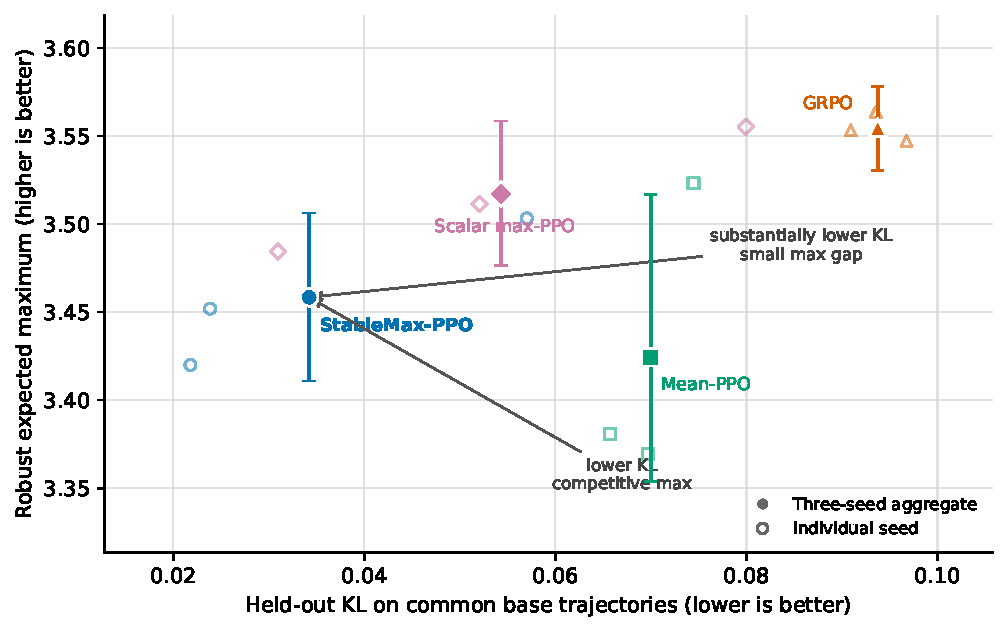
\includegraphics[width=0.60\linewidth]{figures/max_kl_pareto.pdf}
\caption{Robust maximum versus held-out KL. Filled markers are three-seed
aggregates; open markers are individual seeds and bars are 95\% intervals.}
\label{fig:max-kl-pareto}
\end{figure}

Figure~\ref{fig:max-kl-pareto} makes the trade-off explicit: \method{} has
lower held-out KL than all three trainable primary comparators while retaining a
competitive robust maximum, whereas the max-oriented comparators remain higher
on that endpoint.
Rollback frequency is an optimization diagnostic, not a population guarantee.

The aggregate numbers quantify the operating point rather than a universal
ranking.  Relative to Mean-PPO, \method{} increases robust maximum by 0.034
while reducing held-out KL from 0.070 to 0.034 (a 51\% relative reduction).
Relative to Scalar max-PPO, it gives up 0.059 robust-max points while using
0.020 less KL.  These are the two axes that the method exposes; collapsing them
into one weighted score would conceal the engineering trade-off the experiment
is designed to measure.

The comparison should be read as an operating-point result, not as evidence
that the safeguards make every endpoint larger.  GRPO and Scalar max-PPO
demonstrate that more aggressive max-seeking can reach a higher target-RM
maximum under this protocol, but their larger held-out KL records the additional
policy movement.  StableMax-PPO instead reaches a nearby point with lower
drift, which is the behavior predicted by treating quality and motion as
constraints rather than as unreported side effects.

\subsection{Ablation and stability analysis}
\label{subsec:ablation-stability-main}
The component variants isolate changes to the target from changes to the
controller.  Removing the mean floor raises the aggregate robust maximum from
\(3.458\) to \(3.508\), but also raises held-out KL from \(0.034\) to \(0.048\).
Removing the independent-quality floor gives the operating point
\((3.467,0.048)\), while removing calibration robustification gives
\((3.421,0.028)\), in (robust maximum, held-out KL) coordinates.  The
three-seed intervals overlap and the per-seed effects are heterogeneous, so
these comparisons are sensitivity analyses rather than isolated causal
effects.  In particular, removing calibration changes the evaluator-defined
target, whereas removing a floor changes the accepted-update trajectory.  The
complete aggregate and per-seed tables are in
Appendix~\ref{app:full-experiments}; no component is presented as a universally
improving reward term.

Together, the results answer the objective-design question at the evaluated
operating point: the robust ordinal credit trains against the same
finite-budget statistic used for evaluation, while quality floors and held-out
KL keep typical performance and policy movement visible.  Independent
generated-output diagnostics are reported in
Appendix~\ref{subsec:anti-exploitation}; they are model-based diagnostics
rather than fresh human judgments.

\section{Limitations}
\label{sec:limitations}
\textbf{Scope.} The endpoint is induced by frozen evaluators, with no fresh human
labels for generated outputs; model proxies may disagree with people, the
1.5B/14B capacity gap may induce evaluator shift, and three seeds do not
establish scale or domain generalization.  We fix \(N=32\), and the exact
product form assumes conditionally independent rating outcomes, so correlated
annotation or evaluator errors are outside the guarantee.

\textbf{Future work.} Blinded human ratings, additional response budgets and
domains, larger policies, and correlated-error ambiguity sets are natural next
tests.  The last direction is especially important because it asks whether the
threshold construction can retain tractable policy credit when evaluator errors
are shared across candidates.

\emph{Reproducibility statement.} The supplementary artifact contains the
source, official ICLR style files, protocol, result tables, verification JSON,
build commands, and the anonymous repository at
\url{https://github.com/LoveGuys-cmd/rlhf-artifact}.  The main paper specifies
the objective, algorithm, seeds, metrics, and aggregate results; appendices
give proofs and the complete protocol.  Model weights, credentials, private
data, and other non-redistributable files are excluded.

\emph{AI use statement.} Generative AI tools assisted with paper
organization, methodological exposition, language editing, LaTeX and figure
formatting, and debugging of analysis code.  The authors independently checked
all mathematical claims and proofs, verified implementation and numerical
values against frozen result files, and reviewed every AI-assisted change.  No
AI system generated experimental data or replaced author verification.

\emph{Ethics statement.} The study uses model-generated text and existing
preference data.  It collects no new human-subject data or personal
information.  Model-based preference proxies are reported as proxies, not as
human judgments of newly generated outputs; possible reward-model exploitation
and evaluator shift are disclosed in Section~\ref{sec:limitations} and
Appendix~\ref{app:full-experiments}.
\label{main-text-end}
\bibliographystyle{iclr2027_conference}
\bibliography{references}
\appendix
\emph{Appendix roadmap.}
Appendix A gives the ordinal parameterization and proofs of the exact objective,
calibration, gradient, variance, and rollback claims.  Appendix B records the
complete experimental protocol and diagnostics; Appendix C gives implementation
conventions for Algorithm~\ref{alg:stablemax}; machine-readable hashes and
verification records are summarized at the end of Appendix C.
\makeatletter
\renewcommand{\theHtable}{appendix.\arabic{table}}
\renewcommand{\theHfigure}{appendix.\arabic{figure}}
\renewcommand{\theHalgocf}{appendix.\arabic{algocf}}
\makeatother

\section{Detailed theoretical analysis}
\label{app:theory}

\subsection{Ordinal-probit parameterization}
\label{app:ordinal-probit}
Write \(\Delta(\mathcal R)\) for the probability simplex on
\(\mathcal R=\{0,1,2,3,4\}\).
The frozen Moment RM emits a latent location $m_\omega(x,y)$ and positive
scale $s_\omega(x,y)$.  With frozen cutpoints
$c_1<\cdots<c_4$, its five-category probabilities are
\(p_{\omega,0}=\Phi((c_1-m_\omega)/s_\omega)\),
\(p_{\omega,r}=\Phi((c_{r+1}-m_\omega)/s_\omega)-
\Phi((c_r-m_\omega)/s_\omega)\) for $r=1,2,3$, and
\(p_{\omega,4}=1-\Phi((c_4-m_\omega)/s_\omega)\).  The moments used by
the policy are \(\mu_\omega=\sum_{r=0}^4rp_{\omega,r}\) and
\(\sigma_\omega^2=\sum_{r=0}^4(r-\mu_\omega)^2p_{\omega,r}\).
Repeated-rating likelihood and disagreement supervise the conditional scale;
therefore this variance is a model-based signal of annotation disagreement,
not epistemic uncertainty or a stand-alone reward.  Proper scoring and
calibration are required because the complete categorical distribution enters
the finite-budget objective \citep{mccullagh1980regression,kendall2017uncertainties,
lou2024uncertainty,sun2025purm,gneiting2007strictly,guo2017calibration}.

This parameterization is included to make the evaluator interface reproducible,
not to claim a new ordinal-link model.  The methodological choice is what the
policy does with the frozen output: the same five probabilities support the
nominal mean, threshold products, robust envelope, and disagreement diagnostic.
Keeping these uses separate is important because replacing the vector by its
mean would make the finite-budget objective and its calibration check
unidentifiable.

\begin{proposition}[Finite-support threshold decomposition]
\label{prop:threshold-decomposition}
For conditionally independent ratings supported on
\(\mathcal R=\{0,1,2,3,4\}\),
the identity
\(h_N^{\rm nom}=\sum_{t=1}^{4}[1-\prod_{j=1}^{N}F_{\omega,j}(t-1)]\)
is exact, lies in \([0,4]\), and is nondecreasing under first-order stochastic
improvement of any candidate.  Its highest-threshold component is
\(1-\prod_j(1-p_{\omega,4}(x,Y_j))\).
\end{proposition}

The proposition is the finite-support sanity check for the main construction.
It also explains why the top-rating diagnostic in the artifact is not a
substitute for the reported objective: it is only the \(t=4\) term, whereas the
method trains against all four threshold events.  This distinction prevents a
policy from appearing successful by concentrating probability only at the
highest category while degrading the intermediate ordinal structure.

\begin{proof}
For any integer-valued \(Z\in\{0,\ldots,4\}\), the tail-sum identity gives
\(\mathbb E[Z]=\sum_{t=1}^{4}\Pr\{Z\ge t\}\).  Taking
\(Z=\max_jR_j\) and using (A1) gives
\(\Pr\{\max_jR_j<t\mid x,Y_{1:N}\}=\prod_{j=1}^{N}F_{\omega,j}(t-1)\).

Substitution proves the stated nominal identity.  Each term lies in
\([0,1]\), so the sum lies in \([0,4]\).  First-order
stochastic improvement decreases a candidate CDF and therefore cannot
decrease any summand.  At \(t=4\),
\(F_{\omega,j}(3)=1-p_{\omega,4}(x,Y_j)\), giving the highest-threshold
expression above.
\end{proof}

\begin{proposition}[Prompt-cluster calibration statement]
\label{prop:calibration-radius}
Assume that the validation prompt clusters are independent and that the
reward model is fixed before they are evaluated.  For cluster \(g\), let
\(R_{g\ell}\) denote its repeated ratings, \(n_g\) its number of ratings, and
\(F_{\omega,g\ell}(t)\) the frozen evaluator CDF at threshold \(t\).  Define
\(D_{g,t}=n_g^{-1}\sum_{\ell=1}^{n_g}
\{\mathbf{1}[R_{g\ell}\le t]-F_{\omega,g\ell}(t)\}\) for
\(t=0,\ldots,3\), and let
\(\widehat d_t=G_{\mathrm{cal}}^{-1}\sum_{g=1}^{G_{\mathrm{cal}}}D_{g,t}\), where
\(G_{\mathrm{cal}}\) is the number of independent validation clusters.  Let
\(\mathbb E_g\) denote expectation over the validation-cluster distribution.
Define the calibration radius as
\begin{equation}
\label{eq:epsilon-calibration}
\varepsilon_{\rm cal}
=
\min\!\left\{
1,\,
\max_{t=0,\ldots,3}(\widehat d_t)_+
+
\sqrt{
\frac{\log(4/\alpha_{\rm cal})}
     {2G_{\rm cal}}
}
\right\}.
\end{equation}
Then, with probability at least \(1-\alpha_{\rm cal}\),
\[
\mathbb E_g[D_{g,t}]\le\varepsilon_{\rm cal}
\qquad
\text{simultaneously for }t=0,1,2,3.
\]
\end{proposition}

\begin{proof}
Conditional on the frozen responses and predictions, changing all binary
indicators in a prompt cluster from zero to one changes \(D_{g,t}\) by
at most one.  Thus each cluster residual lies in an interval of width one.
Hoeffding's inequality gives
\(\Pr(\mathbb E_g[D_{g,t}]-\widehat d_t>
\sqrt{\log(4/\alpha_{\mathrm{cal}})/(2G_{\mathrm{cal}})})
\le\alpha_{\mathrm{cal}}/4\).

A union bound over four thresholds proves the simultaneous event.  On that
event, every right-hand side is bounded by the unclipped expression in
\cref{eq:epsilon-calibration}.  If clipping is active,
\(\varepsilon_{\mathrm{cal}}=1\), while
\(\mathbb E_g[D_{g,t}]\le1\), so the claim still holds.
\end{proof}

\emph{Scope of the calibration proposition.}
\Cref{prop:calibration-radius} is a population-average statement over the
validation prompt distribution, not a distribution-free pointwise guarantee
for every generated response.  The calibration split fixes the radius before
training, whereas the main theorem is conditional on its envelope covering a
particular candidate; the artifact records these two claims separately.

\begin{proof}[Proof of Theorem~\ref{thm:main-max}]
The envelope \(\overline F_j\) is nondecreasing, has boundary values zero and one, and therefore defines a valid categorical distribution. For every feasible \(q_j \in \mathcal U\), we have
\[
F_{q_j}(t) \le \overline F_j(t), \qquad t = 0,1,2,3.
\]
Hence \(q_j\) first-order stochastically dominates \(\overline p_j\), or equivalently \(\overline p_j\) is the stochastically smallest distribution in the ambiguity set. Since the maximum is coordinatewise nondecreasing in its ratings, replacing every feasible candidate distribution by \(\overline p_j\) cannot increase its expectation. The envelope itself is feasible and thus attains the infimum. Applying \Cref{prop:threshold-decomposition} gives the stated closed form.
\end{proof}

\begin{proof}[Proof of Theorem~\ref{thm:main-gradient}]
For nonnegative integer ratings, the positive-part marginal credit can be decomposed as
\[
(\overline R_i-\overline M_{-i})_+ = \sum_{t=1}^{4} \mathbf{1}\{\overline R_i \ge t,\; \overline M_{-i} < t\}.
\]
Taking conditional expectations and using the conditional independence assumption (A1) gives
\[
\Pr\{\overline R_i \ge t,\; \overline M_{-i} < t \mid x,Y_{1:N}\}
=
[1-\overline F_i(t-1)] \prod_{j \ne i} \overline F_j(t-1),
\]
which proves \Cref{eq:robust-credit-closed}.

For the gradient identity, fix \(i\) and condition on \((x, Y_{-i})\). The robust group value decomposes as
\[
h_N^{\mathrm{rob}} = \mathbb E[\overline M_{-i} \mid x, Y_{-i}] + q_i^{\mathrm{rob}}.
\]
The first term is independent of \(Y_i\), and the score-function identity implies that its product with \(\nabla_\theta \log \pi_\theta(Y_i \mid x)\) has conditional expectation zero. Applying the likelihood-ratio derivative to all \(N\) i.i.d. responses and summing the remaining terms proves \Cref{eq:robust-policy-gradient}.
\end{proof}

\begin{proof}[Proof of Theorem~\ref{thm:coverage-summary}]
Under (A1), let \(F_j^*\) denote the true conditional CDF. Under the pointwise
coverage premise \(F_j^*(t) \le \overline F_j(t)\) for every candidate and
threshold, first-order stochastic dominance directly yields the lower-bound
inequality stated in Theorem~\ref{thm:coverage-summary}. The same independence
assumption permits the product comparison used for the misspecified case.

For the misspecified case, define
\[
\xi \triangleq \max_{j,t}\, [F_j^*(t) - \overline F_j(t)]_+.
\]
At each threshold, the true and robust tail-sum terms can differ only through the corresponding CDF products. For arbitrary \(a_j, b_j \in [0,1]\), the product difference is bounded by the sum of positive differences:
\[
\prod_j a_j - \prod_j b_j \le \sum_j (a_j - b_j)_+.
\]
Applying this inequality with \(a_j = F_j^*(t-1)\) and \(b_j = \overline F_j(t-1)\) at each of the four thresholds, the discrepancy is at most \(N\xi\) per threshold, and therefore at most \(4N\xi\) after summation. Taking outer expectations preserves the resulting inequality:
\[
\mathbb E_*[\max_j R_j] \ge h_N^{\mathrm{rob}} - 4N\xi.
\]
\end{proof}

\begin{proof}[Proof of Proposition~\ref{prop:radius-monotonicity}]
Fix a candidate group and threshold \(t\), and define
\[
a_j(\varepsilon) \triangleq \min\{1,\; F_{\omega,j}(t-1) + \varepsilon\}.
\]
For \(0 \le \varepsilon_1 \le \varepsilon_2 \le 1\), the clipping map is nondecreasing and 1-Lipschitz, which gives
\[
0 \le a_j(\varepsilon_2) - a_j(\varepsilon_1) \le \varepsilon_2 - \varepsilon_1.
\]
Using the telescoping product identity and the fact that \(a_j(\varepsilon) \in [0,1]\), we have
\[
0 \le \prod_j a_j(\varepsilon_2) - \prod_j a_j(\varepsilon_1)
\le \sum_j \bigl(a_j(\varepsilon_2) - a_j(\varepsilon_1)\bigr)
\le N(\varepsilon_2 - \varepsilon_1).
\]
Substituting this bound into the four-term tail-sum expression for \(h_N^{\mathrm{rob}}\), and then taking expectations over prompts and responses, proves Proposition~\ref{prop:radius-monotonicity}.

At \(\varepsilon = 0\), the robust envelope equals the nominal CDF, so the exact infimum in Theorem~\ref{thm:main-max} equals \(J_N^{\mathrm{nom}}(\theta)\).
\end{proof}

\begin{proof}[Proof of Proposition~\ref{prop:variance}]
By the conditional credit definition in \Cref{eq:robust-credit-closed}, we have
\[
\mathbb E[(\overline R_i-\overline M_{-i})_+ \mid x, Y_{1:N}] = q_i^{\mathrm{rob}},
\]
for every \(i\). The score terms \(\phi_i\) are fixed under this conditioning, so linearity gives
\[
\mathbb E[G_{\mathrm{samp}} \mid x, Y_{1:N}] = G_{\mathrm{RB}}.
\]
For any fixed vector \(v\), the law of total variance yields
\[
\mathrm{Var}(v^\top G_{\mathrm{samp}})
=
\mathbb E\bigl[\mathrm{Var}(v^\top G_{\mathrm{samp}} \mid x, Y_{1:N})\bigr]
+
\mathrm{Var}(v^\top G_{\mathrm{RB}}),
\]
which directly implies the stated variance inequality.
\end{proof}

\begin{proof}[Proof of Proposition~\ref{prop:rollback}]
Let \((\theta_0, \mathsf{Opt}_0)\) denote the snapshot taken before a tentative update. If the measured rollout-state KL exceeds \(\delta_{\mathrm{hard}}\), the algorithm executes the restoration \((\theta, \mathsf{Opt}) \leftarrow (\theta_0, \mathsf{Opt}_0)\). By the semantics of the implementation's state-copy operation, both objects are restored exactly to their pre-update values. Because controller-state updates occur only in the accepted branch, a rejected transition also leaves the baseline, dual variables, KL coefficient, and RMS scale unchanged. This statement is conditional on the measured batch and therefore makes no population-level KL claim.
\end{proof}

\begin{proposition}[\(N=1\) reduction and complexity]
\label{cor:n1-reduction}
For \(N=1\),
\[
h_1^{\mathrm{rob}} = q_1^{\mathrm{rob}} = \sum_{r=0}^{4} r \overline p_{1,r}.
\]
Thus the upper-tail reward component reduces exactly to the robust mean reward. For general \(N\), all group values and marginal credits can be computed in \(O(N|\mathcal R|)\) time using threshold-wise prefix and suffix products.
\end{proposition}

This reduction serves as a useful implementation sanity check: at \(N=1\), the method must recover the robust mean and cannot manufacture a group advantage. For \(N>1\), the additional terms exactly capture the response's incremental chance of opening a new threshold above the other candidates. The test suite validates both regimes, ensuring that any improvement in the group objective cannot be attributed to a special-case implementation artifact.

\begin{proof}
With a single candidate, the empty opponent maximum is zero by convention, so \((\overline R_1 - 0)_+ = \overline R_1\), and the first equality follows directly. For the complexity analysis, note that evaluating each of the four nontrivial thresholds requires one forward and one backward product scan over the \(N\) candidates. Hence the total time is \(O(N \cdot |\mathcal R|)\), where \(|\mathcal R| = 5\).
\end{proof}


\section{Full experimental protocol}
\label{app:full-experiments}

\subsection{Experimental questions}
\label{subsec:experimental-questions}

The experiments are designed to answer four predeclared questions:

\begin{enumerate}
\item Does StableMax-PPO attain a competitive held-out robust
\(\mathbb E[\max_{j\le32}R_j]\) objective relative to
mean optimization and a direct scalar max@32 policy gradient, while
reducing held-out KL?
\item Are gains preserved under the nominal exact ordinal maximum and the
top-rating probability \(\Pr\{\exists j:R_j=4\}\)?
\item Do nominal expected rating, independent Quality RM score, and
reference-policy KL remain within their predeclared safeguards?
\item Do independent generated-output proxies and existing human-labeled
preference diagnostics provide evidence against target-RM exploitation?
\end{enumerate}

No result is used to remove a comparator, redefine a threshold, or select a more
favorable protocol.

\subsection{Protocol audit and scientific interpretation}
\label{subsec:gate-outcomes}

The artifact verifier passed for seeds 314, 2718, and 1618.  The terminal
record preserves every predeclared proxy, non-inferiority, safeguard, and KL
outcome for auditability. We interpret these fields as protocol diagnostics
that characterize the measured operating points, not as a universal method
ranking or a proof that reward-model exploitation is absent.

The diagnostic vector is read as a decision record rather than a single
leaderboard score.  A method can satisfy KL and quality safeguards while
losing a max comparison, or improve the target reward while degrading an
independent proxy.  Reporting the vector preserves these distinctions and
prevents a favorable endpoint from hiding a failure mode that the method was
designed to measure.

The aggregate terminal record reports \texttt{scientific\_success=false}:
the mean and independent-quality floors and the held-out KL comparisons against
Mean-PPO and GRPO pass, but the declared robust-maximum gates and Qwen
proxy gate do not all pass. In particular, the paired robust-maximum difference
from Mean-PPO is 0.0339 with a 95\% interval of $[-0.0686,0.1304]$.
The corresponding intervals against GRPO and Scalar max-PPO are
$[-0.1336,-0.0609]$ and $[-0.1024,-0.0101]$. Passing artifact verification
therefore establishes protocol consistency, not scientific success.

The recorded runs fix \(\varepsilon_{\rm run}=0.04680826120821986\)
using the earlier calibration rule with \(\alpha_{\rm cal}=0.05\).
As explained in Appendix~\ref{app:theory}, this is a fixed ambiguity-set
parameter, not a certified population calibration radius. We retain all
recorded outcomes and do not substitute the corrected formula into completed
runs. The released summaries record the radius; the original cluster-level
calibration data and report remain external, so their sample count and split
independence cannot be reconstructed from this release.

\subsection{Models, data, and split discipline}
\label{subsec:models-data}

The policy is Qwen2.5-1.5B-Instruct
\citep{qwen2024qwen25}.  The frozen Moment RM is a Qwen2.5-14B ordinal
model trained on HelpSteer2 repeated helpfulness ratings, with the
decontaminated preference replay recorded in its training manifest
\citep{wang2024helpsteer2}.  It exports
\(p_{\omega,0:4}\) directly; exposing the category probabilities
does not retrain or alter its accepted checkpoint.  An independently trained
Qwen2.5-14B scalar Quality RM, fit separately on disjoint preference data,
supplies \(Q_\eta\) and has no
variance head.  Its frozen 4,096-pair confirmation accuracy is
\(94.60\%\) with a Wilson lower 95\% bound of
\(93.87\%\).

All policy, reward-model, evaluator, and lockbox splits are content-hashed.
Before partitioning RewardBench, we remove prompt and response overlap with
the policy and Quality-RM data \citep{lambert2024rewardbench}.  The remaining
calibration, policy-diagnostic, and reserve partitions are also mutually
prompt- and response-disjoint.  They contain 1,024, 1,024, and 427 pairs,
respectively.  The sealed Skywork diagnostic contains 4,096 pairs and is
excluded from Quality-RM training and selection
\citep{liu2024skyworkreward}.

The Moment RM and policy prompts remain drawn from the same broad HelpSteer2
domain.  Disjoint rows prevent direct leakage but do not establish
out-of-domain generalization; this is treated as a limitation rather than
hidden by the split terminology.

\subsection{Frozen training protocol}
\label{subsec:experimental-protocol}

The primary response budget is \(N=32\).  Each trainable confirmatory method uses
three seeds \(\{314,2718,1618\}\), 300 policy steps, two prompts
per step, 32 responses per prompt, learning rate \(2\times10^{-5}\),
one PPO epoch, clip \(0.2\), LoRA rank 8 with scale 32, sampling
temperature 1, \(\mathrm{top}_p=1\), maximum prompt length 384,
and maximum response length 64. Seed \(42\) is used only for development and real-GPU smoke tests and is
excluded from all confirmatory intervals, gates, and aggregate claims. The target KL is \(0.02\) and the
hard rollback level is \(0.04\).  All methods share the same prompt
stream, generation budget, optimizer class, policy architecture, and
checkpoint-selection rule.

The non-inferiority floors are frozen before any trainable policy outcome is
observed.  The reference sample contains 2,048 base-policy responses from 512
independent policy-training prompts, with four responses per prompt.  For
\(Z\in\{\mu_\omega,Q_\eta\}\), let
\(\bar Z_g\) be the four-response prompt mean and let
\(L_Z\) be the fifth percentile of 10,000 bootstrap means obtained by
resampling prompts.  The frozen floor is \(z_0=L_Z-0.1s_Z\),
where \(s_Z\) is the response-level standard deviation in the same
reference sample.  The bootstrap unit, one-sided level, 10,000 draws, sample
counts, generation seed, bootstrap seed, and practical margin are all
predeclared.  A separate prompt-disjoint sample of 512 responses from 128
prompts reports standardized reference-policy shift.  It is diagnostic only
and cannot accept or reject training.

\subsection{Comparators and ablations}
\label{subsec:comparators}

The ten trainable methods are:

\begin{enumerate}
\item \textbf{StableMax-PPO}: the complete method in
Algorithm~\ref{alg:stablemax}.
\item \textbf{Mean-PPO + Q}: PPO on
\(\mu_\omega\) with the same mean, Quality, and KL protocol.
\item \textbf{GRPO + Q}: group-relative standardized
\(\mu_\omega\) credit with matched safeguards
\citep{shao2024deepseekmath,guo2025deepseekr1}.
\item \textbf{Scalar Max@32-PPO + Q}: exact leave-one-out scalar
max credit
\( [\mu_i-\max_{j\ne i}\mu_j]_+ \)
with matched safeguards
\citep{tang2025inference,walder2025pkpo,bagirov2025best}.
\item \textbf{Entropic-PPO + Q}: PPO on
\(\mathrm{CE}_{\tau}=-\tau\log\sum_r p_{\omega,r}e^{-r/\tau}\),
using \(\tau=1\).
\item \textbf{Nominal Ordinal EV-PPO + Q}: exact
\(J_{32}^{\mathrm{nom}}\) without the CDF ambiguity set.
\item \textbf{StableMax-PPO without mean floor}: ablates nominal-mean
non-inferiority.
\item \textbf{StableMax-PPO without Quality RM}: ablates the independent
quality safeguard and is excluded from constrained-feasibility claims.
\item \textbf{Gaussian EV-PPO + Q}: the previous heteroscedastic
Gaussian expected-maximum objective, retained as a model-assumption ablation.
\item \textbf{Top-4 PPO + Q}: exact optimization of
\(\Pr\{\exists j:R_j=4\}\), isolating the highest
threshold from the complete ordinal maximum.
\end{enumerate}

An eleventh, evaluation-only \textbf{Best-of-32} row samples 32 responses
from the untrained base policy and ranks them by
\(\mu_\omega\).  It is an inference-time reference, not a
compute-matched training baseline; its generation and scoring cost is reported
separately.

The comparator set is organized to separate three changes that are otherwise
easy to conflate: the deployment functional (mean, scalar maximum, top-rating,
or full ordinal maximum), the CDF robustification, and the stabilizers.
The nominal ordinal and Gaussian variants hold the policy optimizer fixed while
changing the evaluator assumption; the no-floor variants hold the target fixed
while removing one safeguard.  This is why the ablations support a controlled interpretation of the observed
operating points without claiming that any single component is universally
beneficial.

\begin{table}[t]
\caption{Complete aggregate table. Values are three-seed robust expected
maximum, with 95\% confidence intervals, held-out KL, and rollback counts.}
\label{tab:full-aggregate}
\centering\footnotesize
\begin{tabular}{lcccc}
\toprule
Method & Robust max & 95\% CI & Held-out KL & Rollbacks/900\\
\midrule
StableMax-PPO & 3.458 & [3.411, 3.506] & 0.034 & 279 (31.0\%)\\
Mean-PPO & 3.424 & [3.354, 3.517] & 0.070 & 527 (58.6\%)\\
GRPO & 3.555 & [3.530, 3.578] & 0.094 & 741 (82.3\%)\\
Scalar max-PPO & 3.517 & [3.476, 3.558] & 0.054 & 285 (31.7\%)\\
Entropic PPO & 3.400 & [3.353, 3.447] & 0.037 & 302 (33.6\%)\\
Nominal EV-PPO & 3.421 & [3.377, 3.467] & 0.028 & 121 (13.4\%)\\
StableMax-PPO (no mean floor) & 3.508 & [3.426, 3.574] & 0.048 & 230 (25.6\%)\\
StableMax-PPO (no quality floor) & 3.467 & [3.402, 3.530] & 0.048 & 329 (36.6\%)\\
Gaussian EV-PPO & 3.558 & [3.533, 3.581] & 0.061 & 367 (40.8\%)\\
Top-4 PPO & 3.418 & [3.353, 3.499] & 0.042 & 277 (30.8\%)\\
Best-of-32 (base) & 3.086 & [3.045, 3.125] & -- & --\\
\bottomrule
\end{tabular}
\end{table}

\begin{table}[t]
\centering
\footnotesize
\caption{Per-seed primary endpoints at $N=32$. Each cell reports robust
expected maximum / held-out KL on the same 512-prompt evaluation split. The KL
values are the common-base-trajectory means from the held-out evaluator, matching
the aggregate endpoint in Table~\ref{tab:full-aggregate}.}
\label{tab:per-seed-primary}
\begin{tabular}{lccc}
\toprule
Method & Seed 314 & Seed 2718 & Seed 1618 \\
\midrule
StableMax-PPO & 3.503 / 0.057 & 3.452 / 0.024 & 3.420 / 0.022 \\
Mean-PPO & 3.369 / 0.070 & 3.523 / 0.074 & 3.381 / 0.066 \\
GRPO & 3.563 / 0.094 & 3.547 / 0.097 & 3.553 / 0.091 \\
Scalar max-PPO & 3.511 / 0.052 & 3.555 / 0.080 & 3.484 / 0.031 \\
\bottomrule
\end{tabular}
\end{table}

The per-seed view makes the operating-point claim testable without relying on
the aggregate interval alone: StableMax-PPO has lower held-out KL than Mean-PPO
and GRPO in every seed, and lower KL than Scalar max-PPO in two of the three
seeds (2718 and 1618).  Its robust maximum remains competitive across the same paired prompts.
The robust values are the checked-in per-seed CSV records and the KL values are
the held-out common-base means; all entries are rounded only for display, with
no additional aggregation or seed selection performed here.

\subsection{Ablation and stability analysis}
\label{subsec:ablation-stability}

The component rows in Table~\ref{tab:full-aggregate} isolate the operating
point controls.  Removing the mean floor increases the aggregate robust maximum
from \(3.458\) to \(3.508\), but also raises held-out KL from \(0.034\) to
\(0.048\).  Removing the independent Quality floor gives
\((3.467,0.048)\), while removing CDF robustification gives
\((3.421,0.028)\), in (robust maximum, KL) coordinates.  The three-seed
intervals overlap and the per-seed effects are heterogeneous, so these are
sensitivity comparisons rather than isolated causal effects. CDF-envelope
removal changes the evaluator-defined target; floor removal changes the
accepted-update trajectory.  The records therefore support a controlled operating-point interpretation,
not a claim that any safeguard is a universally improving reward term.

\subsection{Evaluation endpoints}
\label{subsec:evaluation-endpoints}

Every method is evaluated on 512 frozen test prompts with newly generated
groups of 32 responses.  The primary paired prompt-level endpoint is
\(h_{32}^{\mathrm{rob}}\), exactly matching the StableMax-PPO
training objective.  Secondary model-based endpoints are
\(h_{32}^{\mathrm{nom}}\),
\(U_{32}^{\mathrm{nom}}\), candidate-level
\(\mu_\omega\), ordinal variance,
\(p_{\omega,4}\), independent Quality score, reference KL,
constraint residuals, accepted updates, and exact rollback counts.

The confirmatory evaluation fixes \(N=32\) for every method; no cross-budget
sensitivity result is claimed.  The group-level maximum uses all 32 candidates
and does not require a selected response.  A deployment-style
\(\arg\max_i\mu_\omega(x,Y_i)\) response is reported only as a secondary
selector diagnostic.  Held-out KL is computed on common base trajectories, so
the paired comparison measures policy motion under the same prompt protocol
rather than differences in test-set difficulty.

For completeness, the top-category diagnostic used in the cached evaluation
is
\begin{equation}
\label{eq:any-four}
U_N^{\mathrm{nom}}(\theta)
:=\mathbb E_{x,Y_{1:N}}\!\left[
1-\prod_{j=1}^{N}(1-p_{\omega,4}(x,Y_j))\right].
\end{equation}
It is the frozen-model probability that at least one candidate receives rating
four.  It is not a Gaussian tail approximation and is not the primary
estimand; the complete ordinal maximum remains the reported objective.

\subsection{Statistical analysis and success criteria}
\label{subsec:statistical-analysis}

All seeds are reported separately. The frozen analysis uses 10,000 draws of
a seed-then-prompt percentile bootstrap: sample three seeds with replacement,
then independently resample 512 prompt indices within each sampled seed.
Paired method contrasts use within-seed prompt differences before resampling.
The resulting 2.5th and 97.5th percentiles are the reported intervals. Because
prompts are shared across seeds but resampled independently within them, these
are intervals under the frozen nested-resampling convention, not an exact
crossed seed--prompt population confidence guarantee. Three seeds further
limit precision of inference over training randomness.

The recorded success gates require the robust-max difference interval's lower
endpoint to be \(>0\) against Scalar max-PPO, \(\ge-0.05\) against
Mean-PPO, and \(\ge-0.10\) against GRPO. They also require the held-out-KL
difference interval's upper endpoint to be \(<0\) against both Mean-PPO and
GRPO. The candidate nominal-mean and Quality-score interval lower endpoints
must reach their respective frozen floors. Each generated-output proxy must
have tie-adjusted preference mean \(\ge0.50\) and interval lower endpoint
\(\ge0.45\). All nine gates must pass jointly; the recorded decision is false.
These are the unchanged protocol criteria, not thresholds chosen after seeing
the results. We make no superiority claim from the positive Mean-PPO
robust-max point estimate.

Additional diagnostics average paired differences over seeds within each
prompt before sign-flip randomization. Such tests require sign-exchangeability
under their null. The historical output key \texttt{paired\_rank\_biserial}
actually records the sign-based effect \((n_+-n_-)/(n_++n_-)\), excluding
zero differences (defined as zero if all differences vanish); it does not
weight signed ranks. We retain that field name for record compatibility and
interpret it as a sign-dominance statistic. Individual intervals and auxiliary
tests are descriptive and are not simultaneous confidence guarantees across
all methods or endpoints.

\subsection{Anti-exploitation and human-grounded diagnostics}
\label{subsec:anti-exploitation}

Newly generated outputs are compared with Mean-PPO outputs by two frozen
evaluators: the Qwen2.5-14B-Instruct judge and
\texttt{RLHFlow/ArmoRM-Llama3-8B-v0.1}
\citep{zheng2023judging,wang2024interpretable}.  For each seed, the diagnostic
aligns up to 512 held-out prompt groups, retains the response selected by
$\arg\max_i\mu_\omega(x,Y_i)$ from each 32-response group, and evaluates the
matched pair.  Qwen judgments use randomized presentation order and a reverse
order check; ArmoRM supplies an independent pointwise score.  Each evaluator
must first pass its frozen RewardBench calibration gate (between 512 and 1,024
calibration pairs, with the frozen split and hashes recorded by the protocol).
Pairwise judgments are model-based proxies, not human labels.  The complete
group-level diagnostic is run separately on all 32 candidates and reports
robust/nominal maximum, probability of any rating-4 response, and the paired
group delta; selected-response diagnostics additionally report length,
character count, repeated-trigram rate, unique-word ratio, refusal behavior,
and upper-tail strata.

\begin{table}[H]
\caption{Independent generated-output proxy comparisons against Mean-PPO.
Preference is tie-adjusted, so $0.5$ denotes parity; intervals are three-seed
hierarchical-bootstrap 95\% intervals.}
\label{tab:proxy-diagnostics}
\centering\footnotesize
\begin{tabular}{lcc}
\toprule
Evaluator & Preference & 95\% CI\\
\midrule
Qwen2.5-14B judge & 0.494 & [0.478, 0.510]\\
ArmoRM-Llama3-8B-v0.1 & 0.502 & [0.458, 0.544]\\
\bottomrule
\end{tabular}
\end{table}

Both point estimates are near parity and both intervals contain 0.5. These
intervals establish neither a quality difference nor equivalence to Mean-PPO;
in particular, the Qwen proxy does not pass its declared gate.  A
target-RM increase accompanied by proxy degradation would be evidence
consistent with reward-model exploitation; these results do not show that
signature, but the model-based design cannot establish its absence.

RewardBench and Skywork chosen--rejected lockboxes contain previously collected
human labels.  For each policy, length-normalized chosen--rejected policy
log-probability accuracy and margin are reported as preference-retention
diagnostics.  They are not Best-of-32 endpoints and do not label newly sampled
policy responses.  In particular, a new response cannot be declared human
preferred merely because it was generated for a prompt that also appears in a
fixed preference benchmark.

No new human annotation is collected in this protocol.  Therefore, even if
all anti-exploitation gates pass, the permitted claim is
\emph{no evidence of exploitation under the measured model-based and
existing-label diagnostics}.  The experiment cannot establish absence of
reward hacking or direct human preference for generated outputs.  A blinded
group-rating packet is emitted so that fresh human evaluation can be added
later without regenerating or selecting outputs.

\subsection{Reproducibility and reporting}
\label{subsec:reproducibility}

Code, model adapters, data partitions, floor samples, calibration reports, and
protocol files are content-hashed before training.  A real-GPU smoke test must
execute every declared objective, verify finite applicable metrics, verify
constraint activation, and test exact parameter and optimizer rollback.
Formal training and evaluation run only after these checks pass.  Technical
failures are versioned and corrected with regression tests.  Unfavorable
scientific outcomes are reported without changing seeds, thresholds,
comparators, evaluators, or success criteria.

The 1.5B policy is evaluated by 14B reward and proxy models.  This capacity
gap may improve discrimination but may also create systematic evaluator shift.
The three-seed design measures optimization variability; it does not replace
replication at other model scales or fresh blinded labels.

\clearpage
\section{Implementation Details for \method}
\label{app:algorithm}

This appendix records implementation conventions for Algorithm~\ref{alg:stablemax},
rather than a second algorithm. Appendix~\ref{app:full-experiments} specifies
models, seeds, and thresholds; the machine-readable supplement provides
aggregate and per-seed tables, terminal records, and SHA-256 hashes.

For each prompt $x_b$, the implementation caches behavior-policy token log
probabilities and response masks before the tentative policy update. The five
ordinal probabilities are converted to prefix CDFs. For
$t=0,\ldots,3$, the robust envelope is
\(\bar F_{b,i}(t)=\min\{1,F_{\omega,b,i}(t)+\varepsilon\}\),
with \(\bar F_{b,i}(-1)=0\) and \(\bar F_{b,i}(4)=1\).
The robust probabilities are adjacent differences of this envelope. Prefix
and suffix products compute all group values and leave-one-out credits in
$O(BN|\mathcal R|)$ time without enumerating rating tuples.

The constrained credit used by the PPO surrogate is
\(\tilde q_{b,i}=q^{\rm rob}_{b,i}+\lambda_m\mu_\omega(x_b,Y_{b,i})/N+
\lambda_qQ_\eta(x_b,Y_{b,i})/N\), with
\(A_{b,i}=N[\tilde q_{b,i}-b_\psi(x_b)]\).
The prompt baseline is fitted only from accepted transitions. Dual variables
use projected updates after acceptance; rejected steps leave all controller
state unchanged. The lagged RMS scale is computed from accepted credits only,
so a rejected outlier cannot change the next normalization factor.

Before the optimizer step, the implementation snapshots all trainable policy
parameters and the complete optimizer state, including momentum and adaptive
variance buffers. It evaluates full-categorical token KL on the same rollout
states after the tentative step. If the hard threshold is exceeded, both
snapshots are restored and no baseline, dual, KL-controller, or RMS state is
advanced. This is an exact batch-level rollback invariant; it does not imply
a population KL bound.

\begin{table}[H]
\centering
\footnotesize
\caption{Implementation invariants checked by the artifact.}
\label{tab:implementation-audit}
\begin{tabular}{p{0.24\linewidth}p{0.46\linewidth}p{0.20\linewidth}}
\toprule
Component & Invariant & Test coverage \\
\midrule
Ordinal kernel & Five probabilities form a valid distribution; CDF boundaries and threshold identities hold. & \texttt{evrl\_ordinal} \\
Credit kernel & Prefix/suffix products match the exact credit and the \(N=1\) reduction. & \texttt{evrl\_reduction} \\
Rollback state & Policy parameters and optimizer buffers are restored together after rejection. & \texttt{publication\_v8} \\
Controller state & Baseline, dual, KL, and RMS states advance only on accepted updates. & \texttt{publication\_v8} \\
Protocol integrity & Finite metrics, content hashes, and verification records are checked before aggregation. & v8 verification \\
\bottomrule
\end{tabular}
\end{table}

\newpage
\subsection{Loss normalization, KL estimands, and controller updates}
Let \(B\) be the number of prompts, \(L_{b,i}\) a sampled response length,
and \(T=\sum_{b,i}L_{b,i}\) the number of action tokens. With
\(\ell_{b,i,h}=\min\{\rho_{b,i,h}A_{b,i},
\operatorname{clip}(\rho_{b,i,h},1-\epsilon_{\rm PPO},1+\epsilon_{\rm PPO})A_{b,i}\}\),
the minimized loss in the recorded implementation is
\[
\mathcal L_k=\frac{-\frac1{BN}\sum_{b,i}\sum_{h=1}^{L_{b,i}}\ell_{b,i,h}
+\frac{\beta_k}{T}\sum_{b,i}\sum_{h=1}^{L_{b,i}}k_\theta(s_{b,i,h})}
{s_k+10^{-8}}.
\]
The policy term sums tokens within a response and averages responses; the KL
term averages all action tokens. States are sampled from \(\pi_{\rm old}\),
and their distribution is held fixed during the surrogate step. Thus the
penalty is not an unbiased gradient of the population \(K(\theta)\).
The post-step rollback statistic uses these same states with updated policy
probabilities. Held-out KL instead averages token KL within each common
base-policy response, then averages those response means within prompts and
across prompts and seeds. Its state distribution and length weighting differ
from the training statistic, so held-out KL may exceed \(\delta_{\rm hard}\)
without contradicting rollback correctness.

After acceptance, for \(Z\in\{\mu_\omega,Q_\eta\}\) and its floor \(z_0\),
\(\lambda_Z\leftarrow\operatorname{clip}(\lambda_Z+0.05(z_0-\widehat Z),0,20)\),
where \(\widehat Z\) averages the accepted rollout's candidate scores and
both duals start at one. Let \(c_{b,i}=\widetilde q_{b,i}-b_\psi(x_b)\).
The lagged scale starts at \(s_0=1\), with \(v_0=1\), and updates as
\(v_{k+1}=0.99v_k+0.01(BN)^{-1}\sum_{b,i}c_{b,i}^2\),
\(s_{k+1}=\sqrt{v_{k+1}+10^{-8}}\). The baseline fits the prompt mean of
\(\widetilde q\) by squared loss, with AdamW learning rate \(10^{-3}\) and
hidden width 128. Policy and baseline gradient norms are clipped at one.
The KL coefficient starts at 0.02, doubles when accepted-batch KL exceeds
\(1.5\delta\), halves when it falls below \(\delta/1.5\), and is clipped
to \([10^{-5},10]\). A rejected transition changes none of these states.
The recorded protocol uses one PPO epoch per tentative update.

All floating-point reductions use deterministic tensor order where supported.
The supplementary code contains tests for ordinal identities, credit
reductions, finite metrics, protocol hashes, and rollback restoration.

\end{document}
